\documentclass{article}
\usepackage[english, russian]{babel}
\usepackage{cmap}
\usepackage[table]{xcolor}
\usepackage{graphicx}
\usepackage{color}
\usepackage{subcaption}
\usepackage[export]{adjustbox}
\usepackage{cite}
\usepackage[inline]{enumitem}
\usepackage{hyperref}
\usepackage{mathptmx}
\usepackage[utf8x]{inputenc}

\begin{document}
\selectlanguage{english}
\begin{center}
\textbf{NATIONAL RESEARCH UNIVERSITY HIGHER SCHOOL OF ECONOMICS}

\vspace{20mm}
\textit{Faculty of Computer Science}\\

Bachelor’s Programme “HSE and University of London Double Degree Programme in Data Science and Business Analytics”

\vspace{50mm}
\textbf{Software project report}

“Sentiment Analysis based on Glamping Reviews from TripAdvisors: Developing a Decision-Making Assistant”

\vspace{50mm}
\textbf{Student:} Prokhorova Anastasiia

\vspace{5mm}
\textbf{Supervisor:} Chuvilina Anna

\vspace{20mm}
\end{center}
\begin{center}
    \textbf{28.05.2022}
\end{center}

\renewcommand*\contentsname{Table of contents}
\newpage
\tableofcontents
\newpage

\begin{abstract}
Nine out of ten users, when thinking about buying a product or service, do not know which company to contact. Then people begin to look for the necessary information on the Internet and read the reviews of those who have already interacted with the company. Such a study was conducted by Uberall. Reviews are a strong motivator to buy: 88\% of users trust them in the same way as the recommendations of friends.

With the help of feedback, the client can explain why he will contact your company again or, on the contrary, will not come again. It is important to understand why brands fall in love with some, and do not return to others, and how to build a business strategy in such a way as to develop and improve the service. To do this, you need to assess customer’s level of excitement.

Text analytics and opinion mining find numerous applications in e-commerce, marketing, advertising, politics, market research and any other research.

Sentiment analysis is part of the Natural Language Processing (NLP) techniques that consists in extracting emotions related to some raw texts. This is usually used on social media posts and customer reviews in order to automatically understand if some users are positive or negative and why.
\end{abstract}

\newpage

\section{The object of research}
% \setcounter{section}{1}
Reviews of the TripAdvisors website users, who did glamping in Russia.

\section{The result}
% \setcounter{section}{1}
\textit{The main result} of the project is an attempt to create the recommendation system. This project proposes to develop a sentimental analysis using machine learning tools based on real up-to-date data received by the guests. We should parse the website in order to extract the data needed, highlight emotionally colored words and expressions and analyze them with the respect to the tonality of the words. Finally, we need to develop the frequency analysis of the texts and visualize to the user the “word cloud.”

\section{Basic keywords}
% \begin{flushleft}
\underline{Glamping}  -- a style of camping with amenities and resort-style services not usually associated with "traditional" camping. Glamping has become particularly popular with 21st century tourists seeking the luxuries of hotel accommodation alongside "the escapism and adventure recreation of camping" \newline \newline
\underline{Sentiment analysis} is a method of recognizing and classifying opinions from a piece of text in order to establish whether the writers' attitude toward a given topic or product is positive, negative, or neutral.\newline\newline
\underline{A machine learning model} is a computer software that has been taught to identify specific patterns. The model is trained on a specific data set using an algorithm that allows the data to be analyzed and the findings to be memorized.\newline\newline
\underline{Recommendatory system} -- a software that uses machine learning models to forecast which things will be of interest to the user based on his personal information.\newline\newline
\underline{A dataset} is a collection of raw data that will be used to train and test a machine learning algorithm.\newline\newline
\underline{Text semantics} -- a direction that considers the substantive side of the text, structuring meanings expressed explicitly and implicitly.\newline\newline
\underline{Implicit information} -- information that does not constitute the direct meaning of the text components (words, etc.). Implicit information serves to express the implicit meaning of a text or statement, the hallmark of which is the non-necessity of receiving it on understanding, its incomplete restoration to the listeners.\newline\newline
\underline{Explicit information} -- information derived from the meaning of words in the text or statement that are presented in the dictionary and therefore understandable to the recipient. Explicit information in the text can be presented in the form of explicit statements, which mean statements that carry information directly derived from the dictionary meanings of words used in the statement, that is, those whose content can be established from the superficial form of the statement without directly carrying out additional semantic transformations.\newline\newline
\underline{Tokenization} -- dividing phrase into a different set of statements/dividing a statement into different set of words.\newline\newline
\underline{Cleaning the data} -- removing the special characters/words that do not create any value to the analytics part.


\Huge
$\newline\sqrt{\frac{1}{n}(a_{1}^2+a_{2}^2+\cdots+a_{n}^2)}\vspace{15mm} $ \newline
\LARGE
$\vspace{10mm}\sum_{i=1}^{n}i=\frac{n(n+1)}{2} \vspace{20mm}$ \\
\Huge
$\lim_{h\to 0}\frac{f(x+h)-f(x)}{h}\vspace{10mm}$
\newline
\huge
$\int_0^2\frac{\frac{n(n+1)+\frac{f(x+h)-f(x)}{h}}{2}}{\sqrt{\frac{1}{n}(a_{1}^2+a_{2}^2+\cdots+a_{n}^2)}}$


\normalsize
\newpage
\section{Introduction}
\subsection{Subject area}
\setcounter{section}{4}
Subject area: sentiment analysis

\subsection{Relevance}
\setcounter{section}{4}
Sentiment analysis of hotels is now used\cite{duchin2009markowitz} in the creation of recommendation systems by most hotels around the world. At present, given the current geopolitical situation, the analysis of user reviews from Russia is the most relevant for tourism businesses. Due to limited flights, nature trips within the country are becoming more popular among consumers.

The project will allow to make an optimal decision on the choice of the place to stay for glamping, making the process of surfing more comfortable. It will also give students participating in the project a lot of experience in data science to use in the future. 

\subsection{Goal}
\setcounter{section}{4}
Develop a recommendatory system for glamping tourism based on customer’s feedback.

\subsection{Tasks}
\setcounter{section}{4}

\begin{itemize}[noitemsep]
	\item Examine possible approaches to the task, study tourism market
	\item Find and collect reviews of the customers of places they have stayed in 
	\item Find the main components of ratings using uncontrolled learning to process natural language.
	\item Predict ratings with controlled training based on specific feedback.
	\item Develop a recommendatory system for glamping tourism
\end{itemize}

\newpage
\section{Comparative analysis of sources and analogues}
There exists quite many sentiment analysis of hotel reviews from different parts of the world\cite{markopoulos2015sentiment}. For instance, sentiment analysis of hotel reviews from Booking.com\cite{elnagar2018hotel}. The dataset contains 515,000 customer reviews and scoring of 1493 luxury hotels across Europe with the geographical location of hotels provided.

Despite the fact that there are no direct analogues of our work, there are similar works on hotels in Europe. The principle of sentiment analysis based on hotel reviews and glamping reviews differ. It is important to keep in mind differences between hotel rooms and apartments outside. These differences may influence the thematic vocabulary of users.

Due to the novelty of the glamping tourism there are no direct analogues of sentimental analysis of glamping tourism in Russia. 

Let’s compare our project with the sentiment analysis on tweeter reviews. \newline

\begin{tabular}{|m{2cm}|b{4cm}|p{4cm}|}
\hline
 & Sentiment analysis on glamping reviews & Sentiment analysis 
 on tweeter reviews\cite{philander2016twitter} \\ \hline
 Availability of a ready-made dataset & Need to collect data & Already has the dataset \\ \hline
 Importing libraries & NLTK, Scikit-learn, WordCloud, Dostoevsky, RuSentiment, Pandas, NumPy & NLTK, Scikit-learn, WordCloud, Pandas, Numpy \\ \hline
 Simple preprocessing step & Has & Has \\ \hline
 Lemmatization step & Yes & Yes \\ \hline
 Stemming step & No & No \\ \hline
 Visualization through WordClouds & Yes & Yes \\ \hline
 Evaluation function & Yes & Yes \\ \hline
 Modeling & Yes & Yes \\ \hline
 User interface & Yes & No \\ \hline
\hline
\end{tabular} 
\newline\newline

\rowcolors{1}{yellow}{orange}
\begin{tabular}{m{4cm} m{3cm} m{3cm}}
    \textbf{Characteristics} &  \textbf{Sentiment analysis based on Glamping reviews from TripAdvisors: a decision-making assistant} & \textbf{Twitter Sentiment Analyzer}\cite{ahmad2022urdu}\\ 
    \textbf{Paid/free} & Free & Paid \\ \hline
    \textbf{Visualization} & Option to get sentiment via mind maps, wordclouds and graphs & Option to get sentiment expressed via short video clips \\ \hline 
    \textbf{Function of calculating the rating of an object based on reviews} & No & Yes \\ \hline
    & \multicolumn{2}{|c|}{Extremely simple and intuitive UI} \\ \hline
    \textbf{Used for} & Analyzing glamping places in Russia before travelling & Analyzing the product reviews before buying, analyze trends at stock market, get sentiments on trending \\ 
\end{tabular}
\newline\newline
As we can see the inner methods of sentiment analysis on tweeter and glamping reviews are mostly the same. The significant difference is in data preprocessing and data collection steps.\cite{patel2020sentiment}

\newpage
\section{Description of functional and non-functional requirements}
\subsection{Functional requirements}
\setcounter{section}{6}
\begin{itemize}
    \item An ideal glamping market portfolio is made up of the recommendation system, which includes machine learning algorithms.
    \item The recommendation system should allow to consider the present status of your portfolio and provide solutions for changing it.
\end{itemize}

\subsection{Non-functional requirements}
\setcounter{section}{6}
\begin{itemize}
    \item The system should be easily scalable:
    \begin{itemize}
        \item Uploading the dataset
        \item Choosing places, that analysis the user wants to receive
    \end{itemize}
\end{itemize}
\section{Roles of other members of the project}
The project is implemented by two members. Another participant beside me is Morozova Milena. She is also a 2nd year bachelor degree student at HSE university on faculty of computer science. Our educational program is called “Data science and business analytics”. The role of Milena was dedicated to the creation of the user-friendly interface of the recommendation system. While my task in the project was dedicated to the backend development. In particular, I was to prepare the ready-to-use dataset and collect the data needed for doing the analysis. Moreover, tokenization, cleaning the data, lemmatization, and classification were also in my competence. Together we discussed and implemented machine learning methods.

\newpage
\section{Models, algorithms and methods}
The main purpose of sentiment analysis is to find opinions in a text.\cite{tran2019measuring}

One-dimensional emotive space is most typically utilized in current systems for automatically detecting the emotional assessment of a text: positive or negative. The fundamental goal of sentiment analysis is to determine if a document's or sentence's polarity is positive, negative, or neutral.

The polarity of the text can be determined in several ways, the main ones are: classification on a binary scale, on a multi-band scale, the use of scaling systems, identification of subjectivity/objectivity. 

In our work we rely on an automated sentiment analysis. Since the project is to evaluate the comments of vacation spots, I think it will be most effective to use supervised machine learning. It lies in the fact that at the first stage, a machine classifier is trained on pre-marked texts, and then the resulting model is used when analyzing new documents. There are a number of dictionaries needed by computer programs for sentiment analysis. Among them are WordNet-Affect, SentiWordNet, SenticNet.

MeaningCloud Sentiment Analysis API  works with unstructured texts to determine the tone. The API identifies the tonality locally for individual phrases, establishes a relationship between them to determine the general tonality of the text.

Solves problems such as determining irony in a sentence, determines whether a sentence is a subjective opinion or an objective fact, distinguishes between opposite\cite{duchin2009markowitz} or ambiguous points of view. Tonality analysis can occur both at the level of an entire document and on its individual aspects in any of the ten supported languages. Despite the fact, that the library does not work with Russian language, we have studied the way it works. 

For steps of tokenization, cleaning data, lemmatization, and stemization I have used the most widely used NLTK library.

The Python package for NLP approaches is NLTK (Natural Language Toolkit). NLTK is a popular Python programming language for working with human language data. It includes a set of text processing tools for categorization, tokenization, stemming, tagging, parsing, and semantic reasoning, as well as wrappers for industrial-strength NLP libraries and easy-to-use interfaces to over 50 corpora and lexical resources like WordNet.

For text vectorization and convenient work with machine learning models, we used the Scikit-learn library.

Scikit-learn is a Python package for machine learning. Scikit-learn is a Python-based machine learning package that is available for free. It includes support-vector machines, random forests, gradient boosting, k-means, and DBSCAN, among other classification, regression, and clustering techniques, and is designed to work with the Python numerical and scientific libraries NumPy and SciPy.\cite{srinivasa2018natural}

TextBlob is another great library to word with. It is quiet intuitive and has a lot of tools to operate with. I have studied it additionally in order to apply in this project, however, it works only with English texts. Moreover, it has translation on many different languages, but I got an error while translating all reviews from Russian to English. Probably, this happened because google translate does not support the library anymore. Anyway, knowledge about the work of this library were useful.\cite{gujjar2021sentiment}

\newpage
\section{Project implementation}
\subsection{Preparation step}
\setcounter{section}{9}
\paragraph{Includes:} scraping, gathering data and creating database \newline\newline
The data was gathered from the TripAdvisors website. For this purpose, I used special application called ParseHub, that has a great user-friendly interface and is easy to work with. \newline\newline
This is how the ParseHub looks like: 

\begin{center}
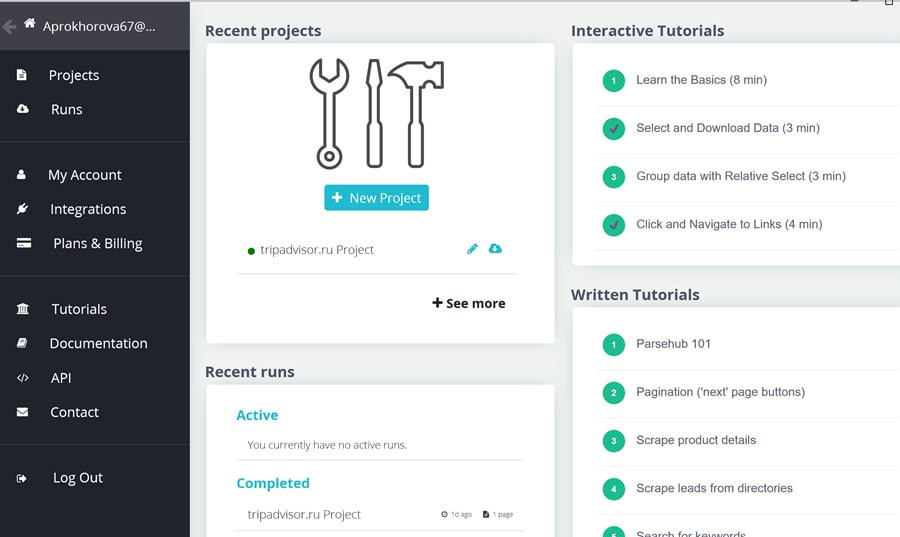
\includegraphics[width=1\linewidth]{images/figure 1.jpg}
\end{center}
\newline\newline
The collected data is a plain text with symbols \{\} and sections ‘places’, ‘section\_1’, and ‘collecting\_comments’ to divide text on readable blocks.
\newline\newline
Here is the way received data looks like:

\begin{figure}
\begin{subfigure}{0.5\textwidth}
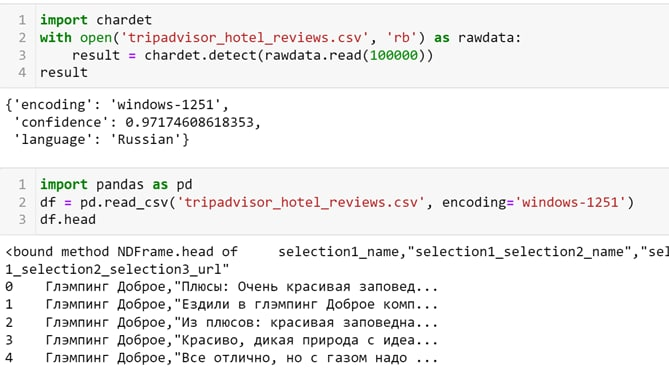
\includegraphics[width=1\linewidth, height=4cm]{images/figure 2.jpg} 
\caption{Caption1}
\label{fig:subim1}
\end{subfigure}
\begin{subfigure}{0.5\textwidth}
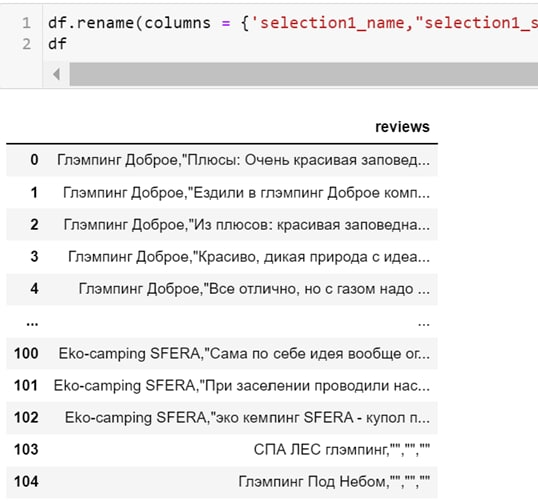
\includegraphics[width=1\linewidth, height=6cm]{images/figure 3.jpg}
\caption{Caption 2}
\label{fig:subim2}
\end{subfigure}
\caption{Data after the \textbf{"preparation step" }}
\end{figure}

\newpage
Dataset was collected from the Tripadvisors website, filtered with ‘glamping in Russia’ pattern. The link: \url{https://www.tripadvisor.ru/Search?q=glamping&searchSessionId=C72C15DF0E5D73ACFC82EB365AF1EDF61644256081930ssid&sid=D9D482CDC580403DAD25CDAEEFAF63BC1644256153605&blockRedirect=true&ssrc=a&geo=294459}

\begin{center}
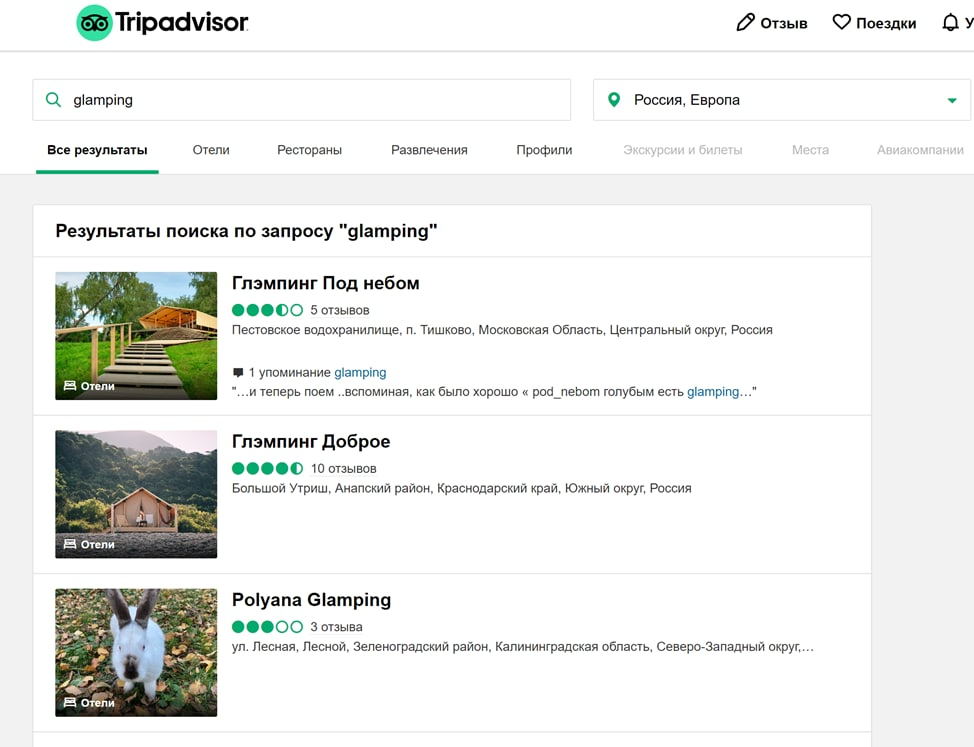
\includegraphics[width=1\linewidth]{images/figure 4.jpg}
\end{center}

\subsection{Preprocessing of data}
\setcounter{section}{9}
\paragraph{Preprocessing of data} is the stage of data mining, which includes the transformation of the source data into an understandable format. \newline
Starting from this stage I have worked with Jupyter Notebook\cite{bressert2012scipy}\cite{harrison2020pandas} as it is a convenient\cite{duchin2009markowitz} way to debug and visualize the problem. The collected data I transformed in the dataframe creating two columns: ‘places’ and ‘collected\_reviews’, where each place has the corresponding\cite{kravets2015creativity} review cell with all collected reviews dedicated to the particular place. There are 30 places in total scrapped from the first page of the website. Each place has review length of about 1800 characters. 
\newpage
The resulting view of the dataframe is as follows:
\newline
\begin{center}
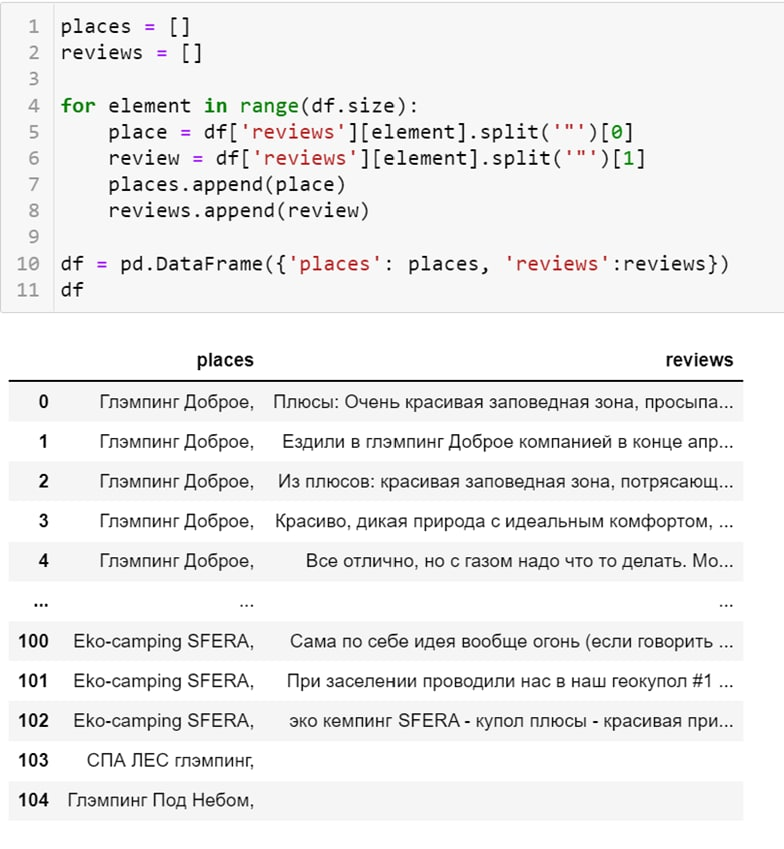
\includegraphics[width=0.7\linewidth, left, height=15cm]{images/figure 5.jpg}
\end{center}
\newline
Before the step of cleaning the received data I split it into two tables: place and reviews. Afterwards, I have united all the reviews to the corresponding places.
\newline
Grouping reviews by places:

\begin{center}
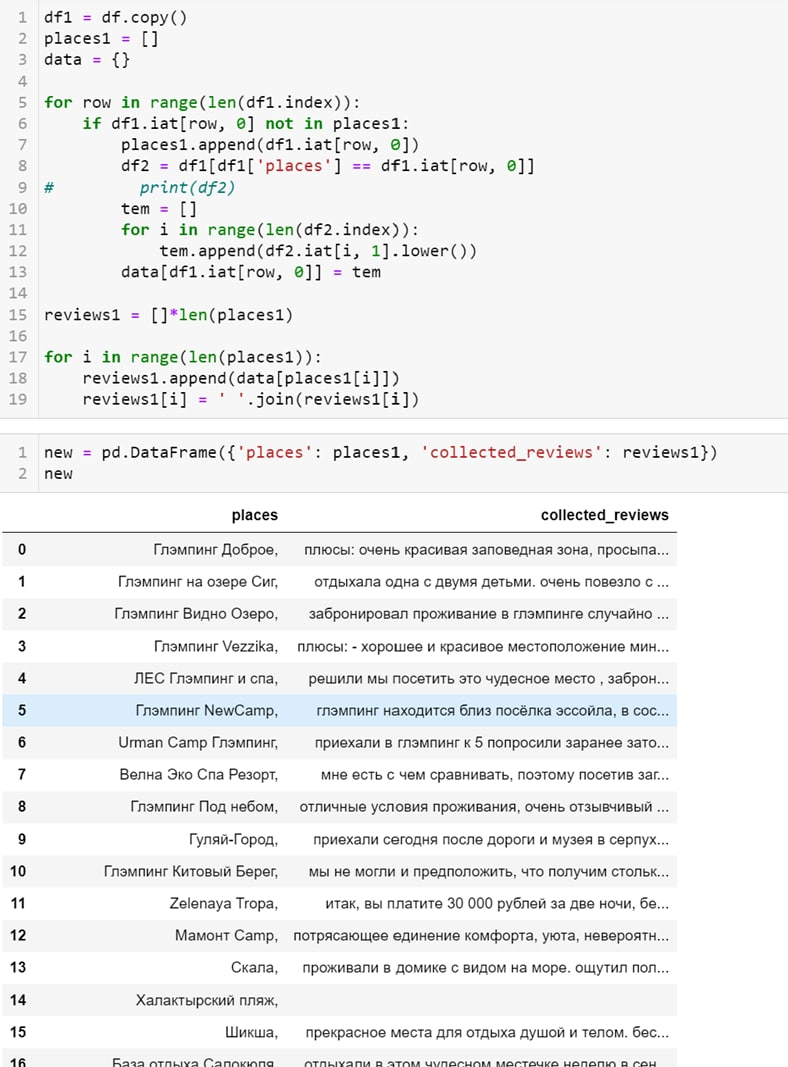
\includegraphics[width=0.5\linewidth, right, height=5cm]{images/figure 6.jpg}
\end{center}

\subsection{Cleaning the data}
\setcounter{section}{9}
\paragraph{Cleaning the data} -- remove the special characters/words that do not create any value to the analytics part.\cite{pradha2019effective}

Going through each word I filtered them with respect to punctuation in strings, special characters and Russian alphabet, because all reviews from the dataset are in Russian language. Thus all the used libraries and methods should be working with Russian texts.\cite{pazelskaya2011method}

\subsection{Tokenization}
\setcounter{section}{9}
\paragraph{Tokenization} -- dividing phrase into a different set of statements/dividing a statement into different set of words.

I used the NLTK library, which is a popular open package of libraries used for various kinds of NLP tasks. Before splitting reviews into words I transformed all the reviews into lower case texts.

\subsection{Removing stop words}
\setcounter{section}{9}
Stop words are frequently used words that do not add any additional information to the text. Words like \selectlanguage{russian} "а", "но", "и" \selectlanguage{english} have no value and only add noise to the data.


The NLTK library has a built-in stopword list that can be used to remove stopwords from text, but I slightly modified it with regard to the working dataset.

\subsection{Lemmatization \& Stemization}
\setcounter{section}{9}

\begin{flushright}
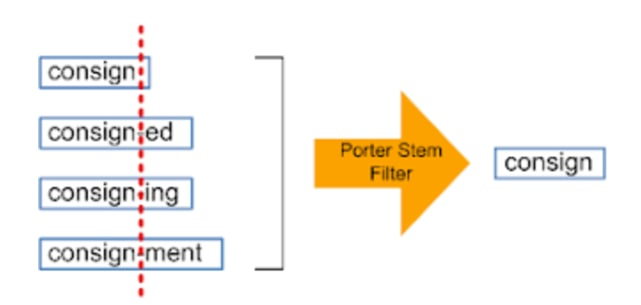
\includegraphics[width=0.5\linewidth, height=5cm]{images/figure 7.jpg}
\end{flushright}
\newline
\underline{Stemization} -- the process of bringing a word to its root/stem. It reduces various variations of a word to its initial form, removes all word appendages and leaves only the base of the word.
\newline
\underline{Lemmatization} is similar to stemization in that it returns the word to its original form, but there is one difference: the root of the term in lemmatization is a word that already exists in the language.
\newline
In our project I applied lemmatization approach as it takes a word into its original lemma, not only the linguistic root of the word. It is also much easier to interpret.
\newline
Cleaning data, tokenization, lemmatization and reducing stop words I have made in one function called ‘preprocessing’:

\begin{center}
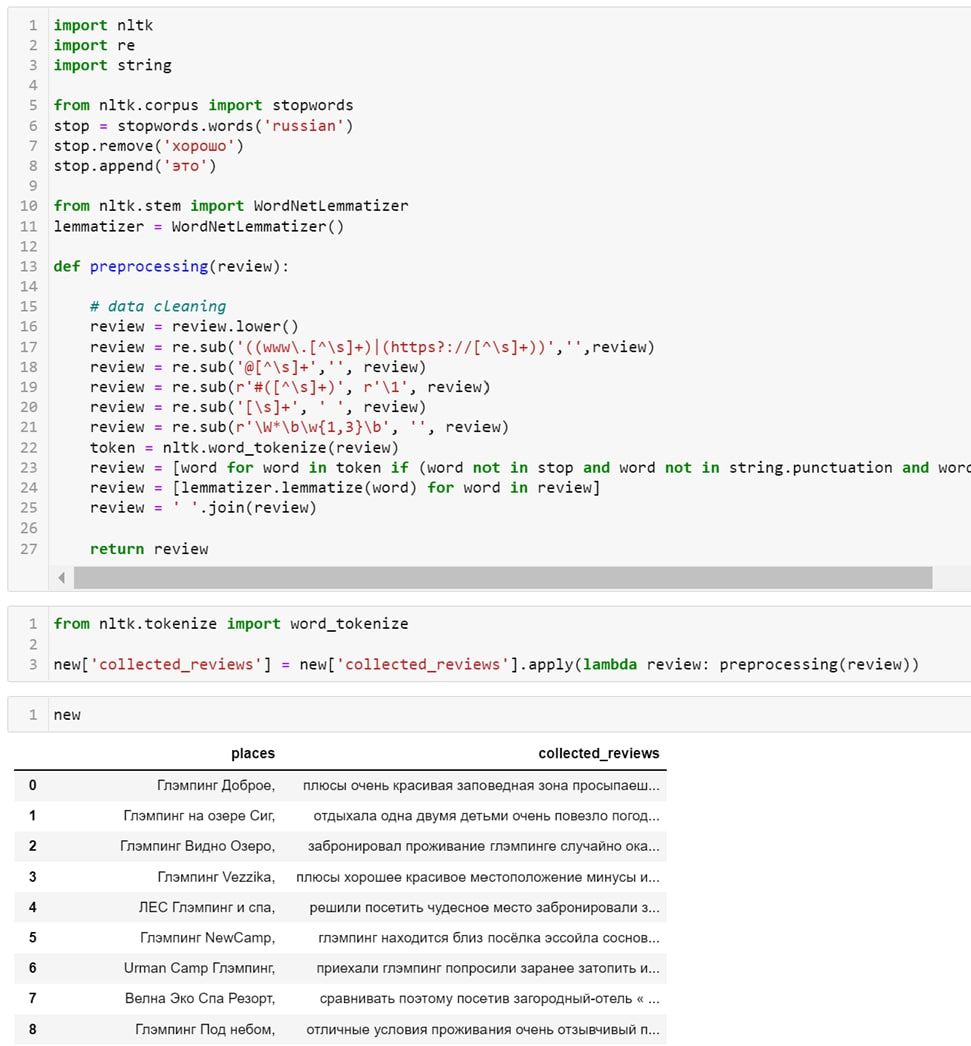
\includegraphics[width=1\linewidth, height=10cm, center]{images/figure 8.jpg}
\end{center}


\subsection{Natural language processing}
\setcounter{section}{9}
For the natural language processing I have used the library called Dostoevsky\cite{sysoev2021studying}. It is an NLP library mostly developed on data from the VK platform. It is based on Russian texts, which is exactly what is analyzed in the project. Moreover, the development team is a native speaker of the Russian language, which accordingly guarantees its best support.\cite{koltsova2016opinion} The library is simple.
\newline
Applying methods from Dostoevsky and RuSentiment libraries I have obtained three sentiments: positive, negative, neutral.\cite{feldman2020behind}


\begin{center}
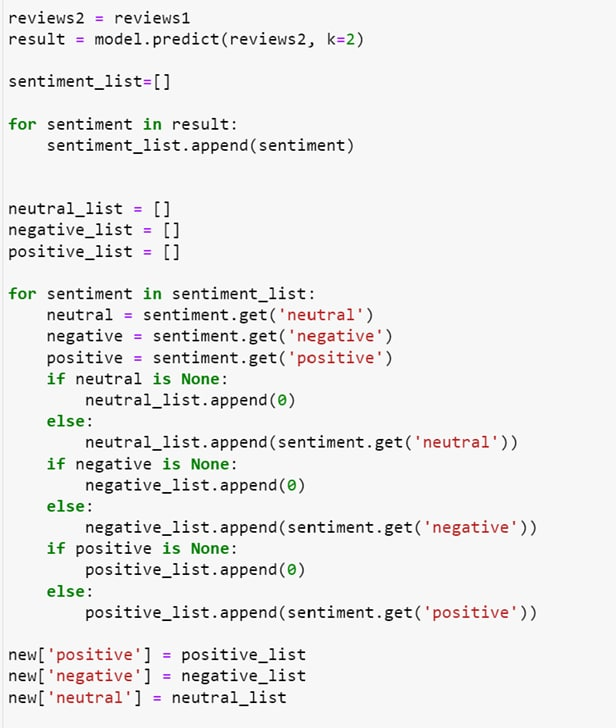
\includegraphics[width=1\linewidth, height=5cm]{images/figure 9.jpg}
\end{center}

The data now is as follows:

\begin{center}
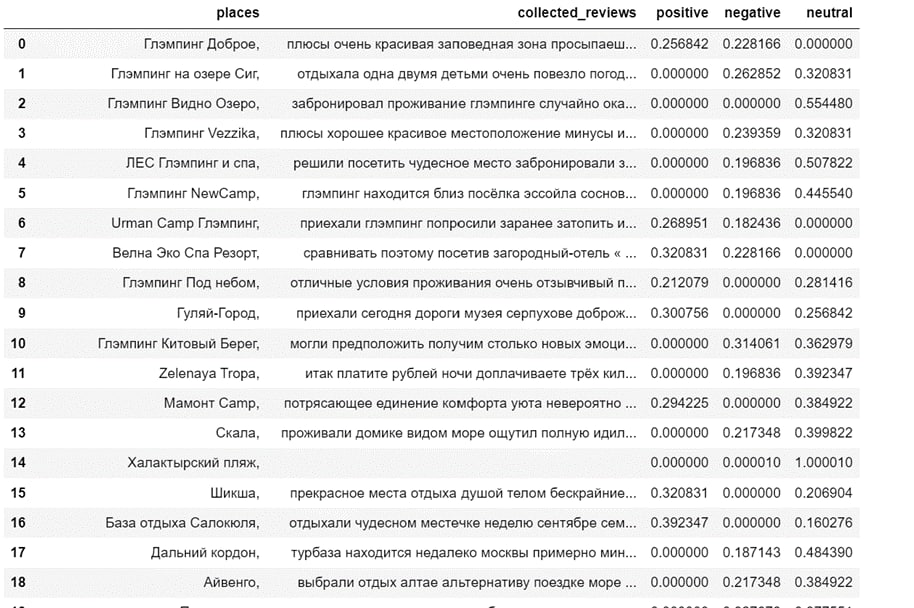
\includegraphics[width=1.2\linewidth, height=7cm]{images/figure 10.jpg}
\end{center}

\newpage
\subsection{Word cloud}
\setcounter{section}{9}
Another interesting pattern I have developed was word clouds. With the help of the WordClouds library. 

Here is the word cloud created for reviews that were positively colored. The column ‘mood’ has two values: 1 and 0, where 1 denotes that the review is more positive than negative or neutral, and 0 – otherwise (negative or neutral).

\begin{center}
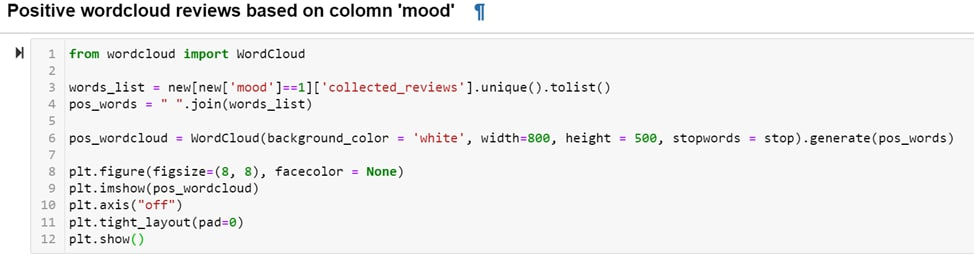
\includegraphics[width=1\linewidth]{images/figure 11.jpg}
\end{center}

As we compare the results for ‘positive’ \textgreater 0 and ‘mood’ == 1, we can say that the assumption underlying the mood column creation was close to results given by the ‘positive’ criteria. 

\begin{center}
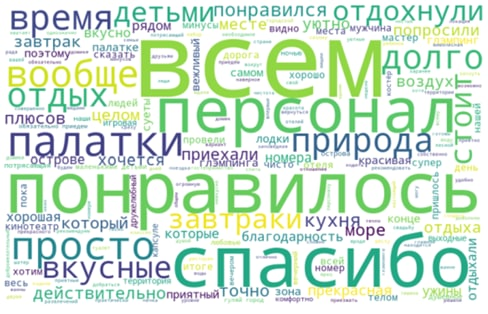
\includegraphics[width=0.4\linewidth,height=5cm]{images/figure 12.jpg}\quad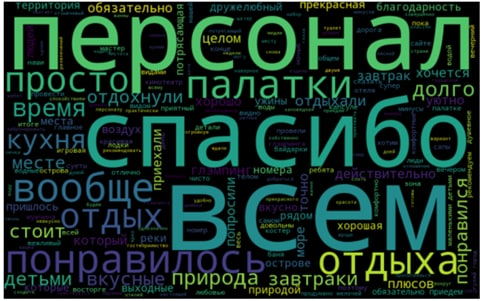
\includegraphics[width=0.4\linewidth,height=5cm]{images/figure 13.jpg}
\end{center}

Summing up the output above, the widely used words in describing the place people liked, were words: \selectlanguage{russian} ‘понравилось’, ‘спасибо’, ‘вкусные’, ‘отдохнули’, ‘прекрасное’, ‘дружелюбный’, ‘хорошая’, ‘плюсов’, ‘потрясающая’, ‘вежливый’, ‘приятный’, ‘довольны’, ‘персонал’. \selectlanguage{english} 

Whereas, more neutral and negative words that do not have any emotional patterns are: \selectlanguage{russian} ‘персонал’, ‘просто’, ‘отдыха’, ‘глэмпинг’, ‘природа’, ‘море’, ‘вода’, ‘минусов’, ‘пляж’, ‘домик’, ‘территория’, ‘ресторан’, ‘мангал’, ‘шатер’. \selectlanguage{english}

\subsection{Text data vectorization}
\setcounter{section}{9}
\paragraph{Text data vectorization} the process of converting text into numbers. 
\newline\newline
Now after text preprocessing, we need to represent the text in numerical form. As an introductory part of machine learning and natural language processing I have tried two ways of vectorising the data: the ‘bag of words’ (BOW) method and TF-IDF method of text vectorization.  In BOW’s logic two sentences are called similar if they consist of the identically the same set of words.

BOW creates a dictionary of unique words in a corpus. Now we can create a table where the columns correspond to the unique words in the corpus and the rows to the sentences. Set the value to 1 if the word is in the sentence, and 0 if it is not there.

Term Frequency & Inverse Document Frequency (TF & IDF). The concept is to weight rare words greater than more frequently used and common words. 

TF calculates the probability of finding a certain word in a document. 

IDF determines the uniqueness of the word in the entire set of reviews.

\subsection{Building model}
\setcounter{section}{9}
After implementing data vectorization we need to build models and check how well and reliably did the model learn. So we built naive Buyers model, naïve Buyes TF-IDF model, and also looked at logistic regression TF-IDF model with the corresponding confusion matrixes.

\newpage
\section{Conclusion}
In this software project I have acquired many useful skills and knowledge especially in such fields as preprocessing data, tokenization, cleaning data, lemmatization, stemization and machine learning processes on an example of Dostoevsky and RuSentiment toolchains. I also got acquainted with NLTK, WordCloud, Skitic-learn libraries, MeaningCloud Sentiment Analysis API. While surfing the net\cite{carreon2021relation} and reading through different researches on sentiment analysis of texts and comments, especially works dedicated to the Russian language texts, I found out that there are not so many libraries and trained models for sentiment analysis in Russian language. Also the process of learning the model is time-consuming and mostly conducted without using already existing word libraries. While doing the project and diving into machine learning techniques, predictions and model construction I have learned of various ways of data vectorization and prediction models application and implementation. Furthermore, the work and skills that have been acquired on this project will be really useful for me in the upcoming academic year and a good bonus in a portfolio for the interview.
\newline\newline
All the materials and source code are stored here: \url{https://github.com/Anastation67/glamping_project_2022.git}

\newpage

\clearpage
\renewcommand*\contentsname{Table of contents}
\addcontentsline{toc}{section}{References}
\bibliographystyle{plain}
\bibliography{bib.bib}


\end{document}


